% Options for packages loaded elsewhere
% Options for packages loaded elsewhere
\PassOptionsToPackage{unicode}{hyperref}
\PassOptionsToPackage{hyphens}{url}
\PassOptionsToPackage{dvipsnames,svgnames,x11names}{xcolor}
%
\documentclass[
  letterpaper,
  DIV=11,
  numbers=noendperiod]{scrartcl}
\usepackage{xcolor}
\usepackage{amsmath,amssymb}
\setcounter{secnumdepth}{-\maxdimen} % remove section numbering
\usepackage{iftex}
\ifPDFTeX
  \usepackage[T1]{fontenc}
  \usepackage[utf8]{inputenc}
  \usepackage{textcomp} % provide euro and other symbols
\else % if luatex or xetex
  \usepackage{unicode-math} % this also loads fontspec
  \defaultfontfeatures{Scale=MatchLowercase}
  \defaultfontfeatures[\rmfamily]{Ligatures=TeX,Scale=1}
\fi
\usepackage{lmodern}
\ifPDFTeX\else
  % xetex/luatex font selection
\fi
% Use upquote if available, for straight quotes in verbatim environments
\IfFileExists{upquote.sty}{\usepackage{upquote}}{}
\IfFileExists{microtype.sty}{% use microtype if available
  \usepackage[]{microtype}
  \UseMicrotypeSet[protrusion]{basicmath} % disable protrusion for tt fonts
}{}
\makeatletter
\@ifundefined{KOMAClassName}{% if non-KOMA class
  \IfFileExists{parskip.sty}{%
    \usepackage{parskip}
  }{% else
    \setlength{\parindent}{0pt}
    \setlength{\parskip}{6pt plus 2pt minus 1pt}}
}{% if KOMA class
  \KOMAoptions{parskip=half}}
\makeatother
% Make \paragraph and \subparagraph free-standing
\makeatletter
\ifx\paragraph\undefined\else
  \let\oldparagraph\paragraph
  \renewcommand{\paragraph}{
    \@ifstar
      \xxxParagraphStar
      \xxxParagraphNoStar
  }
  \newcommand{\xxxParagraphStar}[1]{\oldparagraph*{#1}\mbox{}}
  \newcommand{\xxxParagraphNoStar}[1]{\oldparagraph{#1}\mbox{}}
\fi
\ifx\subparagraph\undefined\else
  \let\oldsubparagraph\subparagraph
  \renewcommand{\subparagraph}{
    \@ifstar
      \xxxSubParagraphStar
      \xxxSubParagraphNoStar
  }
  \newcommand{\xxxSubParagraphStar}[1]{\oldsubparagraph*{#1}\mbox{}}
  \newcommand{\xxxSubParagraphNoStar}[1]{\oldsubparagraph{#1}\mbox{}}
\fi
\makeatother

\usepackage{color}
\usepackage{fancyvrb}
\newcommand{\VerbBar}{|}
\newcommand{\VERB}{\Verb[commandchars=\\\{\}]}
\DefineVerbatimEnvironment{Highlighting}{Verbatim}{commandchars=\\\{\}}
% Add ',fontsize=\small' for more characters per line
\usepackage{framed}
\definecolor{shadecolor}{RGB}{241,243,245}
\newenvironment{Shaded}{\begin{snugshade}}{\end{snugshade}}
\newcommand{\AlertTok}[1]{\textcolor[rgb]{0.68,0.00,0.00}{#1}}
\newcommand{\AnnotationTok}[1]{\textcolor[rgb]{0.37,0.37,0.37}{#1}}
\newcommand{\AttributeTok}[1]{\textcolor[rgb]{0.40,0.45,0.13}{#1}}
\newcommand{\BaseNTok}[1]{\textcolor[rgb]{0.68,0.00,0.00}{#1}}
\newcommand{\BuiltInTok}[1]{\textcolor[rgb]{0.00,0.23,0.31}{#1}}
\newcommand{\CharTok}[1]{\textcolor[rgb]{0.13,0.47,0.30}{#1}}
\newcommand{\CommentTok}[1]{\textcolor[rgb]{0.37,0.37,0.37}{#1}}
\newcommand{\CommentVarTok}[1]{\textcolor[rgb]{0.37,0.37,0.37}{\textit{#1}}}
\newcommand{\ConstantTok}[1]{\textcolor[rgb]{0.56,0.35,0.01}{#1}}
\newcommand{\ControlFlowTok}[1]{\textcolor[rgb]{0.00,0.23,0.31}{\textbf{#1}}}
\newcommand{\DataTypeTok}[1]{\textcolor[rgb]{0.68,0.00,0.00}{#1}}
\newcommand{\DecValTok}[1]{\textcolor[rgb]{0.68,0.00,0.00}{#1}}
\newcommand{\DocumentationTok}[1]{\textcolor[rgb]{0.37,0.37,0.37}{\textit{#1}}}
\newcommand{\ErrorTok}[1]{\textcolor[rgb]{0.68,0.00,0.00}{#1}}
\newcommand{\ExtensionTok}[1]{\textcolor[rgb]{0.00,0.23,0.31}{#1}}
\newcommand{\FloatTok}[1]{\textcolor[rgb]{0.68,0.00,0.00}{#1}}
\newcommand{\FunctionTok}[1]{\textcolor[rgb]{0.28,0.35,0.67}{#1}}
\newcommand{\ImportTok}[1]{\textcolor[rgb]{0.00,0.46,0.62}{#1}}
\newcommand{\InformationTok}[1]{\textcolor[rgb]{0.37,0.37,0.37}{#1}}
\newcommand{\KeywordTok}[1]{\textcolor[rgb]{0.00,0.23,0.31}{\textbf{#1}}}
\newcommand{\NormalTok}[1]{\textcolor[rgb]{0.00,0.23,0.31}{#1}}
\newcommand{\OperatorTok}[1]{\textcolor[rgb]{0.37,0.37,0.37}{#1}}
\newcommand{\OtherTok}[1]{\textcolor[rgb]{0.00,0.23,0.31}{#1}}
\newcommand{\PreprocessorTok}[1]{\textcolor[rgb]{0.68,0.00,0.00}{#1}}
\newcommand{\RegionMarkerTok}[1]{\textcolor[rgb]{0.00,0.23,0.31}{#1}}
\newcommand{\SpecialCharTok}[1]{\textcolor[rgb]{0.37,0.37,0.37}{#1}}
\newcommand{\SpecialStringTok}[1]{\textcolor[rgb]{0.13,0.47,0.30}{#1}}
\newcommand{\StringTok}[1]{\textcolor[rgb]{0.13,0.47,0.30}{#1}}
\newcommand{\VariableTok}[1]{\textcolor[rgb]{0.07,0.07,0.07}{#1}}
\newcommand{\VerbatimStringTok}[1]{\textcolor[rgb]{0.13,0.47,0.30}{#1}}
\newcommand{\WarningTok}[1]{\textcolor[rgb]{0.37,0.37,0.37}{\textit{#1}}}

\usepackage{longtable,booktabs,array}
\usepackage{calc} % for calculating minipage widths
% Correct order of tables after \paragraph or \subparagraph
\usepackage{etoolbox}
\makeatletter
\patchcmd\longtable{\par}{\if@noskipsec\mbox{}\fi\par}{}{}
\makeatother
% Allow footnotes in longtable head/foot
\IfFileExists{footnotehyper.sty}{\usepackage{footnotehyper}}{\usepackage{footnote}}
\makesavenoteenv{longtable}
\usepackage{graphicx}
\makeatletter
\newsavebox\pandoc@box
\newcommand*\pandocbounded[1]{% scales image to fit in text height/width
  \sbox\pandoc@box{#1}%
  \Gscale@div\@tempa{\textheight}{\dimexpr\ht\pandoc@box+\dp\pandoc@box\relax}%
  \Gscale@div\@tempb{\linewidth}{\wd\pandoc@box}%
  \ifdim\@tempb\p@<\@tempa\p@\let\@tempa\@tempb\fi% select the smaller of both
  \ifdim\@tempa\p@<\p@\scalebox{\@tempa}{\usebox\pandoc@box}%
  \else\usebox{\pandoc@box}%
  \fi%
}
% Set default figure placement to htbp
\def\fps@figure{htbp}
\makeatother





\setlength{\emergencystretch}{3em} % prevent overfull lines

\providecommand{\tightlist}{%
  \setlength{\itemsep}{0pt}\setlength{\parskip}{0pt}}



 


\KOMAoption{captions}{tableheading}
\makeatletter
\@ifpackageloaded{tcolorbox}{}{\usepackage[skins,breakable]{tcolorbox}}
\@ifpackageloaded{fontawesome5}{}{\usepackage{fontawesome5}}
\definecolor{quarto-callout-color}{HTML}{909090}
\definecolor{quarto-callout-note-color}{HTML}{0758E5}
\definecolor{quarto-callout-important-color}{HTML}{CC1914}
\definecolor{quarto-callout-warning-color}{HTML}{EB9113}
\definecolor{quarto-callout-tip-color}{HTML}{00A047}
\definecolor{quarto-callout-caution-color}{HTML}{FC5300}
\definecolor{quarto-callout-color-frame}{HTML}{acacac}
\definecolor{quarto-callout-note-color-frame}{HTML}{4582ec}
\definecolor{quarto-callout-important-color-frame}{HTML}{d9534f}
\definecolor{quarto-callout-warning-color-frame}{HTML}{f0ad4e}
\definecolor{quarto-callout-tip-color-frame}{HTML}{02b875}
\definecolor{quarto-callout-caution-color-frame}{HTML}{fd7e14}
\makeatother
\makeatletter
\@ifpackageloaded{caption}{}{\usepackage{caption}}
\AtBeginDocument{%
\ifdefined\contentsname
  \renewcommand*\contentsname{Table of contents}
\else
  \newcommand\contentsname{Table of contents}
\fi
\ifdefined\listfigurename
  \renewcommand*\listfigurename{List of Figures}
\else
  \newcommand\listfigurename{List of Figures}
\fi
\ifdefined\listtablename
  \renewcommand*\listtablename{List of Tables}
\else
  \newcommand\listtablename{List of Tables}
\fi
\ifdefined\figurename
  \renewcommand*\figurename{Figure}
\else
  \newcommand\figurename{Figure}
\fi
\ifdefined\tablename
  \renewcommand*\tablename{Table}
\else
  \newcommand\tablename{Table}
\fi
}
\@ifpackageloaded{float}{}{\usepackage{float}}
\floatstyle{ruled}
\@ifundefined{c@chapter}{\newfloat{codelisting}{h}{lop}}{\newfloat{codelisting}{h}{lop}[chapter]}
\floatname{codelisting}{Listing}
\newcommand*\listoflistings{\listof{codelisting}{List of Listings}}
\makeatother
\makeatletter
\makeatother
\makeatletter
\@ifpackageloaded{caption}{}{\usepackage{caption}}
\@ifpackageloaded{subcaption}{}{\usepackage{subcaption}}
\makeatother
\usepackage{bookmark}
\IfFileExists{xurl.sty}{\usepackage{xurl}}{} % add URL line breaks if available
\urlstyle{same}
\hypersetup{
  pdftitle={Chapter 3 - Multi-parameter models: Exercise solutions},
  pdfauthor={Mattias Villani},
  colorlinks=true,
  linkcolor={blue},
  filecolor={Maroon},
  citecolor={Blue},
  urlcolor={Blue},
  pdfcreator={LaTeX via pandoc}}


\title{Chapter 3 - Multi-parameter models: Exercise solutions}
\author{Mattias Villani}
\date{}
\begin{document}
\maketitle


Click on the arrow to see a solution.

\subsubsection{Exercise 3.1}\label{exercise-3.1}

A dataset contains observations on measurements of pesticide for
\(n=24\) pike fish in a lake in southern Italy. The sample mean
pesticide level is \(\bar{x} = 12.5\) with a sample standard deviation
of \(s=3.1\). Assume that the pesticide levels
\(X_1,\ldots,X_n|\theta,\sigma^2 \sim \mathrm{N}(\theta,\sigma^2)\) are
independent and identically distributed normal random variables with
unknown mean \(\theta\) and unknown variance \(\sigma^2\).

Compute the joint posterior distribution for \(\theta\) and \(\sigma^2\)
using a conjugate prior distribution. Use a prior mean for \(\theta\) of
\(8\) and an (imaginary) prior sample size of \(5\). Use
\(\sigma_0^2 = 1^2\) and \(\nu_0 = 3\) degrees of freedom in your prior
for \(\sigma^2\). Plot the marginal posterior distribution of
\(\theta\).

\begin{tcolorbox}[enhanced jigsaw, title={Solution}, bottomtitle=1mm, opacityback=0, colback=white, colbacktitle=quarto-callout-note-color!10!white, breakable, left=2mm, colframe=quarto-callout-note-color-frame, coltitle=black, bottomrule=.15mm, leftrule=.75mm, toptitle=1mm, titlerule=0mm, arc=.35mm, rightrule=.15mm, opacitybacktitle=0.6, toprule=.15mm]

The posterior distribution is given by \[
\begin{aligned}
\theta | \sigma^2 , \boldsymbol{x} &\sim N\Big(\mu_n,\frac{\sigma^2}{\kappa_n}\Big) \\
\sigma^2 | \boldsymbol{x} &\sim \mathrm{Inv-}\chi^2(\nu_n,\sigma_n^2)
\end{aligned}
\] where \[
\begin{aligned}
\mu_n &= w \bar x + (1-w)\mu_0 \\
w &= \frac{n}{\kappa_0+n} \\
\kappa_n &= \kappa_0 + n \\
\nu_n &= \nu_0 + n  \\
\nu_n\sigma_n^2 &= \nu_0\sigma_0^2 + (n-1)s^2 + \frac{\kappa_0 n}{\kappa_0+n}(\bar x -\mu_0)^2
\end{aligned}
\] We have

\begin{Shaded}
\begin{Highlighting}[]
\CommentTok{\# data }
\NormalTok{n }\OtherTok{=} \DecValTok{24}
\NormalTok{xBar }\OtherTok{=} \FloatTok{12.5}
\NormalTok{s2 }\OtherTok{=} \FloatTok{3.1}\SpecialCharTok{\^{}}\DecValTok{2}

\CommentTok{\# prior}
\NormalTok{mu0 }\OtherTok{=} \DecValTok{8}
\NormalTok{kappa0 }\OtherTok{=} \DecValTok{5}
\NormalTok{nu0 }\OtherTok{=} \DecValTok{3}
\NormalTok{sigma02 }\OtherTok{=} \DecValTok{1}\SpecialCharTok{\^{}}\DecValTok{2}

\CommentTok{\# posterior}
\NormalTok{w }\OtherTok{=}\NormalTok{ n}\SpecialCharTok{/}\NormalTok{(kappa0 }\SpecialCharTok{+}\NormalTok{ n)}
\NormalTok{mun }\OtherTok{=}\NormalTok{ w}\SpecialCharTok{*}\NormalTok{xBar }\SpecialCharTok{+}\NormalTok{ (}\DecValTok{1}\SpecialCharTok{{-}}\NormalTok{w)}\SpecialCharTok{*}\NormalTok{mu0}
\NormalTok{kappan }\OtherTok{=}\NormalTok{ kappa0 }\SpecialCharTok{+}\NormalTok{ n}
\NormalTok{nun }\OtherTok{=}\NormalTok{ nu0 }\SpecialCharTok{+}\NormalTok{ n}
\NormalTok{sigman2 }\OtherTok{=}\NormalTok{ (nu0}\SpecialCharTok{*}\NormalTok{sigma02 }\SpecialCharTok{+}\NormalTok{ (n}\DecValTok{{-}1}\NormalTok{)}\SpecialCharTok{*}\NormalTok{s2  }\SpecialCharTok{+} 
\NormalTok{             (kappa0}\SpecialCharTok{*}\NormalTok{n}\SpecialCharTok{/}\NormalTok{(kappa0 }\SpecialCharTok{+}\NormalTok{ n))}\SpecialCharTok{*}\NormalTok{(xBar }\SpecialCharTok{{-}}\NormalTok{ mu0)}\SpecialCharTok{\^{}}\DecValTok{2}\NormalTok{ )}\SpecialCharTok{/}\NormalTok{nun}
\end{Highlighting}
\end{Shaded}

So the joint posterior is \[
\begin{aligned}
\theta | \sigma^2 , \boldsymbol{x} &\sim N\Big(11.724,\frac{\sigma^2}{29}\Big) \\
\sigma^2 | \boldsymbol{x} &\sim \mathrm{Inv-}\chi^2(27,11.401)
\end{aligned}
\] The marginal posterior for \(\theta\) is \[
\theta \vert \boldsymbol{x} \sim t\Big(\mu_n,\frac{\sigma_n^2}{\kappa_n},\nu_n\Big) = t\Big(27,\frac{11.401}{29},27\Big) 
\] Plotting the marginal posterior of \(\theta\):

\begin{Shaded}
\begin{Highlighting}[]
\NormalTok{thetaGrid }\OtherTok{=} \FunctionTok{seq}\NormalTok{(}\DecValTok{7}\NormalTok{, }\DecValTok{18}\NormalTok{, }\AttributeTok{length =} \DecValTok{1000}\NormalTok{)}
\NormalTok{sigma2Grid }\OtherTok{=} \FunctionTok{seq}\NormalTok{(}\FloatTok{0.001}\NormalTok{, }\DecValTok{30}\NormalTok{, }\AttributeTok{length =} \DecValTok{1000}\NormalTok{)}
\NormalTok{dtdist }\OtherTok{\textless{}{-}} \ControlFlowTok{function}\NormalTok{(x, mu, sigma2, nu)\{}
  \FunctionTok{return}\NormalTok{((}\DecValTok{1}\SpecialCharTok{/}\FunctionTok{sqrt}\NormalTok{(sigma2))}\SpecialCharTok{*}\FunctionTok{dt}\NormalTok{(}\AttributeTok{x =}\NormalTok{ (x }\SpecialCharTok{{-}}\NormalTok{ mu)}\SpecialCharTok{/}\FunctionTok{sqrt}\NormalTok{(sigma2), }\AttributeTok{df =}\NormalTok{ nu))}
\NormalTok{\}}
\FunctionTok{plot}\NormalTok{(thetaGrid, }\FunctionTok{dtdist}\NormalTok{(thetaGrid, mun, sigman2}\SpecialCharTok{/}\NormalTok{kappan, nun), }\AttributeTok{type =} \StringTok{"l"}\NormalTok{, }
     \AttributeTok{xlab =} \FunctionTok{expression}\NormalTok{(theta), }\AttributeTok{ylab =} \StringTok{"posterior density"}\NormalTok{, }
     \AttributeTok{col =} \StringTok{"indianred"}\NormalTok{, }\AttributeTok{main =} \FunctionTok{expression}\NormalTok{(theta))}
\end{Highlighting}
\end{Shaded}

\pandocbounded{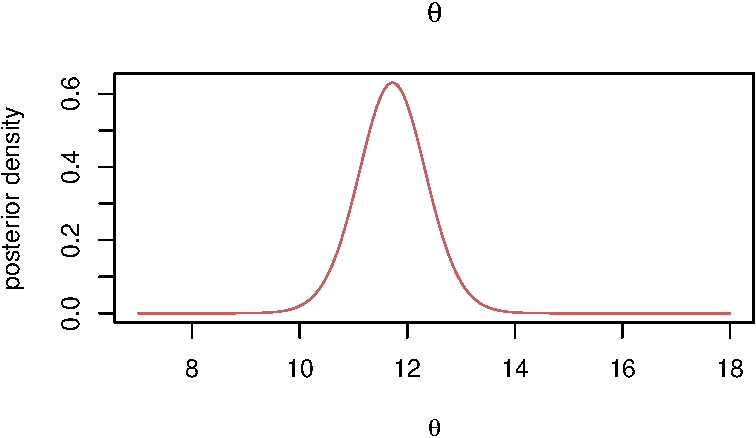
\includegraphics[keepaspectratio]{ch3solutions_files/figure-pdf/unnamed-chunk-3-1.pdf}}

\end{tcolorbox}

\begin{center}\rule{0.5\linewidth}{0.5pt}\end{center}

\subsubsection{Exercise 3.3}\label{exercise-3.3}

Let
\(X_1,\ldots,X_n \mid \theta,\sigma^2 \overset{\mathrm{iid}}{\sim} \mathrm{N}(\theta,\sigma^2)\),
where \(\theta\) is assumed known. Show that the \(\mathrm{Inv-}\chi^2\)
distribution is a conjugate prior for \(\sigma^2\).

\begin{tcolorbox}[enhanced jigsaw, title={Solution}, bottomtitle=1mm, opacityback=0, colback=white, colbacktitle=quarto-callout-note-color!10!white, breakable, left=2mm, colframe=quarto-callout-note-color-frame, coltitle=black, bottomrule=.15mm, leftrule=.75mm, toptitle=1mm, titlerule=0mm, arc=.35mm, rightrule=.15mm, opacitybacktitle=0.6, toprule=.15mm]

The normal density function for a single observation \(x_i\) is \[
 p(x_i \vert \theta, \sigma^2) = \frac{1}{\sqrt{2\pi\sigma^2}}\exp\Big(-\frac{1}{2\sigma^2}(x_i-\theta)^2\Big) \propto \frac{1}{(\sigma^2)^{1/2}}\exp\Big(-\frac{1}{2\sigma^2}(x_i-\theta)^2\Big)
 \] The likelihood for the iid normal model with known mean \(\theta\)
is therefore the product of \(n\) such density functions: \[
 \begin{aligned}
 p(x_1,\ldots,x_n \vert \theta, \sigma^2) = \prod_{i=1}^n p(x_i \vert \theta, \sigma^2) &\propto  \frac{1}{(\sigma^2)^{n/2}}\exp\Big( -\frac{1}{2\sigma^2}\sum_{i=1}^n (x_i-\theta)^2\Big) \\
 &\propto  \frac{1}{(\sigma^2)^{n/2}}\exp\Big( -\frac{n s^2}{2\sigma^2}\Big)
 \end{aligned}
 \] where we have defined
\(s^2 = \frac{\sum_{i=1}^n (x_i-\theta)^2}{n}\) as the sample standard
deviation (dividing by \(n\) instead of \(n-1\) since the mean
\(\theta\) is assumed known).

The density of the
\(\sigma^2 \sim \mathrm{Scaled-Inv-}\chi^2(\nu_0,\sigma_0^2)\) prior is
of the form \[
p(\sigma^2) \propto \frac{1}{(\sigma^2)^{1+\nu_0/2}}\exp\Big( -\frac{\nu_0\sigma_0^2}{2\sigma^2} \Big)
\] The posterior distribution from using the
\(\sigma^2 \sim \mathrm{Scaled-Inv-}\chi^2(\nu_0,\sigma_0^2)\) prior is
given by Bayes' theorem as (to avoid cluttering the notation, we do not
write out the conditioning on \(\theta\) since it is known) \[
\begin{aligned}
p(\sigma^2 \vert x_1,\ldots,x_n) &\propto 
p(x_1,\ldots,x_n \vert \sigma^2)p(\sigma^2) \\
& \propto  \frac{1}{(\sigma^2)^{n/2}}\exp\Big( -\frac{n s^2}{2\sigma^2}\Big) 
\frac{1}{(\sigma^2)^{1+\nu_0/2}}\exp\Big( -\frac{\nu_0\sigma_0^2}{2\sigma^2} \Big) \\
&\propto \frac{1}{(\sigma^2)^{1+(\nu_0+n)/2}}\exp\Big( -\frac{1}{2\sigma^2}\big( \nu_0 \sigma_0^2 + n s^2 \big)  \Big) \\
&=  \frac{1}{(\sigma^2)^{1+(\nu_0+n)/2}}\exp\Big( -\frac{\nu_0+n}{2\sigma^2}\frac{\nu_0 \sigma_0^2 + n s^2 }{\nu_0+n}  \Big)
\end{aligned}
\] which is proportional to a
\(\sigma^2 \sim \chi^2(\nu_0+n,\frac{\nu_0 \sigma_0^2 + n s^2 }{\nu_0+n})\)
density. Note how the location parameter in the posterior \[
\frac{\nu_0 \sigma_0^2 + n s^2 }{\nu_0+n} = \frac{\nu_0}{\nu_0+n} \sigma_0^2 + \frac{n}{\nu_0+n}s^2
\] is a weighted average of prior location \(\sigma_0^2\) and the data
estimate \(s^2\), with more weight placed on the strongest information
source (prior with \(\nu_0\) imaginary sample data points versus the
data with \(n\) actual data points).

\end{tcolorbox}

\begin{center}\rule{0.5\linewidth}{0.5pt}\end{center}

\subsubsection{Exercise 3.6}\label{exercise-3.6}

A Swedish poll in 2024 asked \(2311\) persons the question:
\textit{Which political party would you vote for if there was an election today?}
The table below gives the poll results across the eight parties in
parliament and the nineth option \textit{Other}. \vspace{0.3cm}

\begin{tabular}{lccccccccc}
& M & L & C & KD & S & V & MP & SD & Other \\
\hline 
Votes &      $410$   & $88$    & $83$    & $81$    & $721$   & $196$ & $238$ & $434$ & $60$ \\
Percent & $17.7$ & $3.8$ & $3.6$ & $3.5$ & $31.2$ & $8.5$ & $10.3$ & $18.8$ & $2.6$
\end{tabular}
\vspace{0.3cm}

Let \(\boldsymbol{y} = (y_1,\ldots,y_9)\) denote the number of votes for
each of the nine parties, where \(y_c\) is the number of votes for party
\(c\). Model the data as iid from a multinomial distribution
\begin{equation*}
    \boldsymbol{y} \mid \boldsymbol{\theta} \sim \mathrm{Multinomial}(n,\boldsymbol{\theta}),
\end{equation*} where \(n=2311\) is the total number of respondents and
\(\boldsymbol{\theta} = (\theta_1,\ldots,\theta_9)\) is the vector of
voting proportions for each party, where \(\theta_c\) is the proportion
of votes for party \(c\).

The previous election in 2022 resulted in the following voting
percentages: \vspace{0.3cm}

\begin{tabular}{lccccccccc}
\scriptsize
& M & L & C & KD & S & V & MP & SD & Other \\
\hline 
Percent & $19.1$ & $4.6$ & $6.7$ & $5.3$ & $30.3$ & $6.8$ & $5.1$ & $20.5$ & $1.5$
\end{tabular}
\vspace{0.3cm}

Use Dirichlet prior
\(\boldsymbol{\theta} \sim \mathrm{Dirichlet}(\boldsymbol{\alpha})\)
with \(\boldsymbol{\alpha} = (\alpha_1,\ldots,\alpha_9)\). Set the
priorhyperparameters based on the election results from 2022, but
assuming that the prior information is equivalent to only \(400\)
respondents today.

\begin{enumerate}[(a)]
    \item   \input{exercises/multiparam/multinomial_dirichlet_voting_a.tex}
    \item   \input{exercises/multiparam/multinomial_dirichlet_voting_b.tex}
    \item   \input{exercises/multiparam/multinomial_dirichlet_voting_c.tex}
\end{enumerate}

\textbf{a)} What is the posterior distribution for the voting shares?

\begin{tcolorbox}[enhanced jigsaw, title={Solution}, bottomtitle=1mm, opacityback=0, colback=white, colbacktitle=quarto-callout-note-color!10!white, breakable, left=2mm, colframe=quarto-callout-note-color-frame, coltitle=black, bottomrule=.15mm, leftrule=.75mm, toptitle=1mm, titlerule=0mm, arc=.35mm, rightrule=.15mm, opacitybacktitle=0.6, toprule=.15mm]

Set up data for the current poll, and the results from the election in
2022:

\begin{Shaded}
\begin{Highlighting}[]
\NormalTok{y }\OtherTok{=} \FunctionTok{c}\NormalTok{(}\DecValTok{410}\NormalTok{, }\DecValTok{88}\NormalTok{, }\DecValTok{83}\NormalTok{, }\DecValTok{81}\NormalTok{, }\DecValTok{721}\NormalTok{, }\DecValTok{196}\NormalTok{, }\DecValTok{238}\NormalTok{, }\DecValTok{434}\NormalTok{, }\DecValTok{60}\NormalTok{)}
\NormalTok{election2022 }\OtherTok{=} \FunctionTok{c}\NormalTok{(}\FloatTok{19.10}\NormalTok{, }\FloatTok{4.61}\NormalTok{, }\FloatTok{6.71}\NormalTok{, }\FloatTok{5.34}\NormalTok{, }\FloatTok{30.33}\NormalTok{, }\FloatTok{6.75}\NormalTok{, }\FloatTok{5.08}\NormalTok{, }\FloatTok{20.54}\NormalTok{, }\FloatTok{1.54}\NormalTok{)}
\NormalTok{proportionElection2022 }\OtherTok{=}\NormalTok{ election2022}\SpecialCharTok{/}\DecValTok{100}
\NormalTok{alphaPrior }\OtherTok{=} \DecValTok{400}\SpecialCharTok{*}\NormalTok{proportionElection2022 }\CommentTok{\# not integers, but that\textquotesingle{}s OK}
\end{Highlighting}
\end{Shaded}

Compute the posterior hyperparameters by adding up the data count
\(y_c\) in each category with its corresponding prior count
\(\alpha_c\):

\begin{Shaded}
\begin{Highlighting}[]
\NormalTok{alphaPost }\OtherTok{=}\NormalTok{ alphaPrior }\SpecialCharTok{+}\NormalTok{ y}
\end{Highlighting}
\end{Shaded}

So the (joint) posterior distribution for the Swedish voting shares are
\[
\boldsymbol{\theta} \vert \boldsymbol{y} \sim \mathrm{Dirichlet}\Big(486.4, 106.44, 109.84, 102.36, 842.32, 223, 258.32, 516.16, 66.16\Big)
\]

\end{tcolorbox}

\textbf{b)} What is the marginal posterior distribution for the voting
share of the S-party? Plot the distribution without resorting to
simulation.

\begin{tcolorbox}[enhanced jigsaw, title={Solution}, bottomtitle=1mm, opacityback=0, colback=white, colbacktitle=quarto-callout-note-color!10!white, breakable, left=2mm, colframe=quarto-callout-note-color-frame, coltitle=black, bottomrule=.15mm, leftrule=.75mm, toptitle=1mm, titlerule=0mm, arc=.35mm, rightrule=.15mm, opacitybacktitle=0.6, toprule=.15mm]

From the properties of the Dirichlet distribution box in the Bayesian
Learning book, we know that if
\((\theta_1,\ldots,\theta_C) \sim \mathrm{Dirichlet}(\alpha_1,\ldots,\alpha_C)\),
then marginal distribution for the probability/proportion in category
\(c\) is\\
\[
\theta_c \sim \mathrm{Beta}(\alpha_c, \alpha_+ -\alpha_c).
\] We can apply this result to get the marginal \textbf{posterior} for
\(\theta_5\) (the proportion of S-voters), we just need to remember that
the parameters in the posterior are \(\alpha_c + y_c\) for
\(c=1,\ldots,C\), or \texttt{alphaPost} in the code. The marginal
posterior for the proportion of S-party voters is \[
\theta_5 \vert \boldsymbol{y} \sim \mathrm{Beta}\Big(842.32, 1868.68 \Big),
\] which we can plot:

\begin{Shaded}
\begin{Highlighting}[]
\NormalTok{thetaGrid }\OtherTok{=} \FunctionTok{seq}\NormalTok{(}\DecValTok{0}\NormalTok{, }\DecValTok{1}\NormalTok{, }\AttributeTok{length =} \DecValTok{1000}\NormalTok{)}
\FunctionTok{plot}\NormalTok{(thetaGrid, }\FunctionTok{dbeta}\NormalTok{(thetaGrid, alphaPost[}\DecValTok{5}\NormalTok{], }\FunctionTok{sum}\NormalTok{(alphaPost) }\SpecialCharTok{{-}}\NormalTok{ alphaPost[}\DecValTok{5}\NormalTok{]), }
     \AttributeTok{xlab =} \StringTok{"proportion of S{-}voters"}\NormalTok{, }\AttributeTok{ylab =} \StringTok{"posterior density"}\NormalTok{, }\AttributeTok{type =} \StringTok{"l"}\NormalTok{, }
     \AttributeTok{lwd =} \DecValTok{3}\NormalTok{, }\AttributeTok{col =} \StringTok{"indianred"}\NormalTok{)}
\end{Highlighting}
\end{Shaded}

\pandocbounded{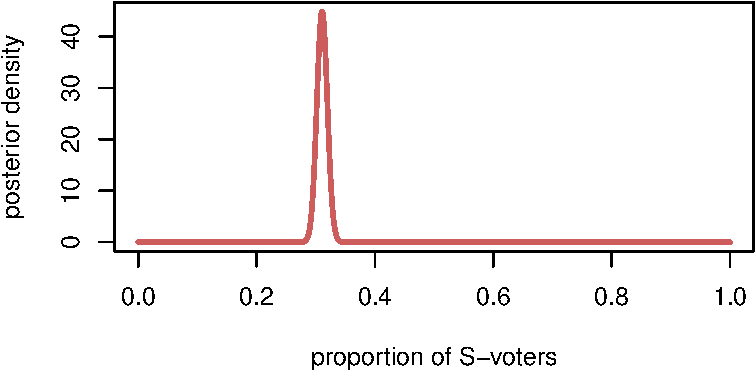
\includegraphics[keepaspectratio]{ch3solutions_files/figure-pdf/unnamed-chunk-6-1.pdf}}

\end{tcolorbox}

\textbf{c)} A party needs at least 4\% of the votes to get into
parliament. Use simulation to compute the posterior probability that
both L and KD parties do not make it to parliament.

\begin{tcolorbox}[enhanced jigsaw, title={Solution}, bottomtitle=1mm, opacityback=0, colback=white, colbacktitle=quarto-callout-note-color!10!white, breakable, left=2mm, colframe=quarto-callout-note-color-frame, coltitle=black, bottomrule=.15mm, leftrule=.75mm, toptitle=1mm, titlerule=0mm, arc=.35mm, rightrule=.15mm, opacitybacktitle=0.6, toprule=.15mm]

Define a Dirichlet random number generator using the algorithm in
Chapter 3.

\begin{Shaded}
\begin{Highlighting}[]
\NormalTok{rdirichlet }\OtherTok{\textless{}{-}} \ControlFlowTok{function}\NormalTok{(nIter, param)\{}
\NormalTok{  nCat }\OtherTok{\textless{}{-}} \FunctionTok{length}\NormalTok{(param)}
\NormalTok{  thetaDraws }\OtherTok{\textless{}{-}} \FunctionTok{matrix}\NormalTok{(}\DecValTok{0}\NormalTok{,nIter,nCat) }\CommentTok{\#Storage}
  \ControlFlowTok{for}\NormalTok{ (j }\ControlFlowTok{in} \DecValTok{1}\SpecialCharTok{:}\NormalTok{nCat)\{}
\NormalTok{    thetaDraws[,j] }\OtherTok{\textless{}{-}} \FunctionTok{rgamma}\NormalTok{(nIter, param[j], }\DecValTok{1}\NormalTok{)}
\NormalTok{  \}}
  \ControlFlowTok{for}\NormalTok{ (i }\ControlFlowTok{in} \DecValTok{1}\SpecialCharTok{:}\NormalTok{nIter)\{}
\NormalTok{    thetaDraws[i,] }\OtherTok{=}\NormalTok{ thetaDraws[i,]}\SpecialCharTok{/}\FunctionTok{sum}\NormalTok{(thetaDraws[i,])}
\NormalTok{  \}}
  \FunctionTok{return}\NormalTok{(thetaDraws)}
\NormalTok{\}}
\end{Highlighting}
\end{Shaded}

Use the simulator to simulate \(10000\) draws from the posterior
distribution. For each draw check if both the L and KD party each have
less than 4\% of the votes.

\begin{Shaded}
\begin{Highlighting}[]
\NormalTok{nSim }\OtherTok{=} \DecValTok{10000}
\NormalTok{postDraws }\OtherTok{=} \FunctionTok{rdirichlet}\NormalTok{(nSim, alphaPost)}
\NormalTok{bothPartyInParliament }\OtherTok{=} \FunctionTok{rep}\NormalTok{(}\ConstantTok{NA}\NormalTok{, nSim)}
\ControlFlowTok{for}\NormalTok{ (i }\ControlFlowTok{in} \DecValTok{1}\SpecialCharTok{:}\NormalTok{nSim)\{}
\NormalTok{  bothPartyInParliament[i] }\OtherTok{=} \FunctionTok{all}\NormalTok{(postDraws[i,}\FunctionTok{c}\NormalTok{(}\DecValTok{2}\NormalTok{,}\DecValTok{4}\NormalTok{)] }\SpecialCharTok{\textless{}} \FloatTok{0.04}\NormalTok{)}
\NormalTok{\}}
\end{Highlighting}
\end{Shaded}

The posterior probability that both parties are below \(4\%\) is 0.4315.

\end{tcolorbox}

\begin{center}\rule{0.5\linewidth}{0.5pt}\end{center}




\end{document}
